\documentclass[twoside]{article}
\usepackage{subcaption}
\input{ISC18-english.sty}
%%%%%%%%%%%%%%%%%%%%%%%%%%%%  Make sure to compile twice for proper cross-references. %%%%%%%%%%%%%%%%%%%%%%%
\begin{document}
\thispagestyle{empty}
%%%%%%%%%%%%%%%%% Article title header  %%%%%%%%%%%%%%%%%%%%
\fancyhead[LE]{Rain Gauge Network Optimization in Khuzestan}
%%%%%%%%%%%%%%%%% Article authors header   %%%%%%%%%%%%%%%%%%%%
\fancyhead[RO]{ Mohammadzadeh and Lotfian }
\begin{center}
{
\includegraphics [height=25mm, width=150.3mm] {Images/isc18E}} \\
\vspace*{-1.8cm}
\vspace*{4cm}
%%%%%%%%%%%%%%%%% Article title  %%%%%%%%%%%%%%%%%%%%
{\Large \bf Spatial Multi-Objective Optimization for Efficient Rain Gauge Network Design in Khuzestan, Iran}\\
%%%%%%%%%%%%%%%%% Article authors and affiliations %%%%%%%%%%%%%%%%%%%%
{\bf
Mohsen Mohammadzadeh\footnote[1]{{\bf Corresponding Author:} {\tt mohsen\_m@modares.ac.ir}}, Elaheh Lotfian\\ 
Department of Statistics, Tarbiat Modares University, Tehran, Iran}
\end{center}
\rule{\textwidth}{0.2mm}\\
%%%%%%%%%%%%%%%%% Article abstract  %%%%%%%%%%%%%%%%%%%%
\noindent{\bf Abstract:}\\
Reliable rainfall monitoring is fundamentally linked to the strategic placement of rain gauge stations; however, many existing networks lack a systematic spatial design. This study introduces a spatial bi-objective optimization framework to evaluate the current rain gauge network in Khuzestan Province, Iran, and to define optimal configurations for future network expansion or restructuring. A novel Hybrid AMOSA\_NSGA-II algorithm is utilized to navigate the trade-off between two competing objectives: minimizing the root mean total error  of rainfall predictions and minimizing the number of stations to reduce operational costs. The results demonstrate that optimized configurations with fewer stations consistently outperform the current network in predictive accuracy. These findings highlight the critical role of spatial optimization in developing cost-effective, high-performance rainfall monitoring systems.
 
\noindent{\bf Keywords:}
Rain gauge station network, Multi-objective optimization, HAN algorithm, Spatial data, Kriging. \\
\noindent{\bf Mathematics Subject Classification (2010):} $\rm 62H11$, $\rm 90C29$, $\rm 62P12$. \\
\hspace{1cm}\rule{\textwidth}{0.2mm}\\
 
%%%%%%%%%%%%%%
\section{Introduction}
 
Rainfall data play a foundational role in water resource management, infrastructure planning, climate change studies, and the forecasting of hydrological extremes such as floods and droughts. In this context, an optimally designed rain gauge network not only enhances the accuracy of rainfall measurements but also minimizes predictive uncertainty and supports informed decision-making—particularly in regions where data coverage is sparse.

The challenge of network design has been addressed through various methodological lenses. \cite{Kar:2015} utilized multi-criteria decision analysis and clustering techniques to identify the most effective rain gauge configurations for flood forecasting in the Mahanadi Basin, India. \cite{Ali:2018} introduced an optimization method integrating cross-validation with geostatistical techniques to prioritize stations under financial constraints, using the root mean square error (RMSE) as the primary optimization criterion. More recently, \cite{Simoyama:2022} explored rain gauge placement to enhance sustainable transportation, while \cite{Simoyama:2023} provided a comprehensive literature review highlighting significant advancements in network optimization. Within Iran, \cite{Zarei:2025} employed a simulation-based approach to design optimal networks for both ungauged plain and mountainous regions.

In Khuzestan Province, Iran, rain gauge stations have historically been installed incrementally without a systematic spatial strategy, potentially compromising the reliability of collected data. This study reformulates the network evaluation as a spatial bi-objective optimization problem, balancing rainfall prediction accuracy against cost reduction. Optimizing multiple conflicting objectives simultaneously results in a Multi-objective Optimization Problem (MOP) \citep{Ehrgott:2005}. To address the inherent limitations of traditional scalarization methods \citep{Fei:2017, Zhu:2006}, we employ the HAN algorithm \citep{Lotfian:2023}, which synthesizes the strengths of AMOSA \citep{Bandyopadhyay:2008} and NSGA-II \citep{Deb:2002} for a robust multi-objective spatial sampling design.
 
\section{Study Area and Dataset}
 
%%%%%%%%%%%%%%%%%%%%%%%%%%%%%%% Figure %%%%%%%%%%%%%%%%%%%%%%%%%%%%%%%%%
Khuzestan Province is located in southwestern Iran, spanning longitudes $47^\circ42'$ to $50^\circ22'$ E and latitudes $29^\circ36'$ to $33^\circ04'$ N, with a total area of approximately $64{,}057\,\text{km}^2$. To account for hydrological continuity and river watersheds that transcend political boundaries, this analysis incorporates a 50-kilometer buffer zone that surrounds the provincial borders. The existing monitoring infrastructure, managed by the Ministry of Energy, consists of 137 rain gauge stations. Figure \ref{fig:location} illustrates the geographical location of Khuzestan Province and the spatial distribution of these stations, with the buffer zone explicitly highlighted in yellow.
\begin{figure}[!ht]
\begin{center}
\subfloat[]
{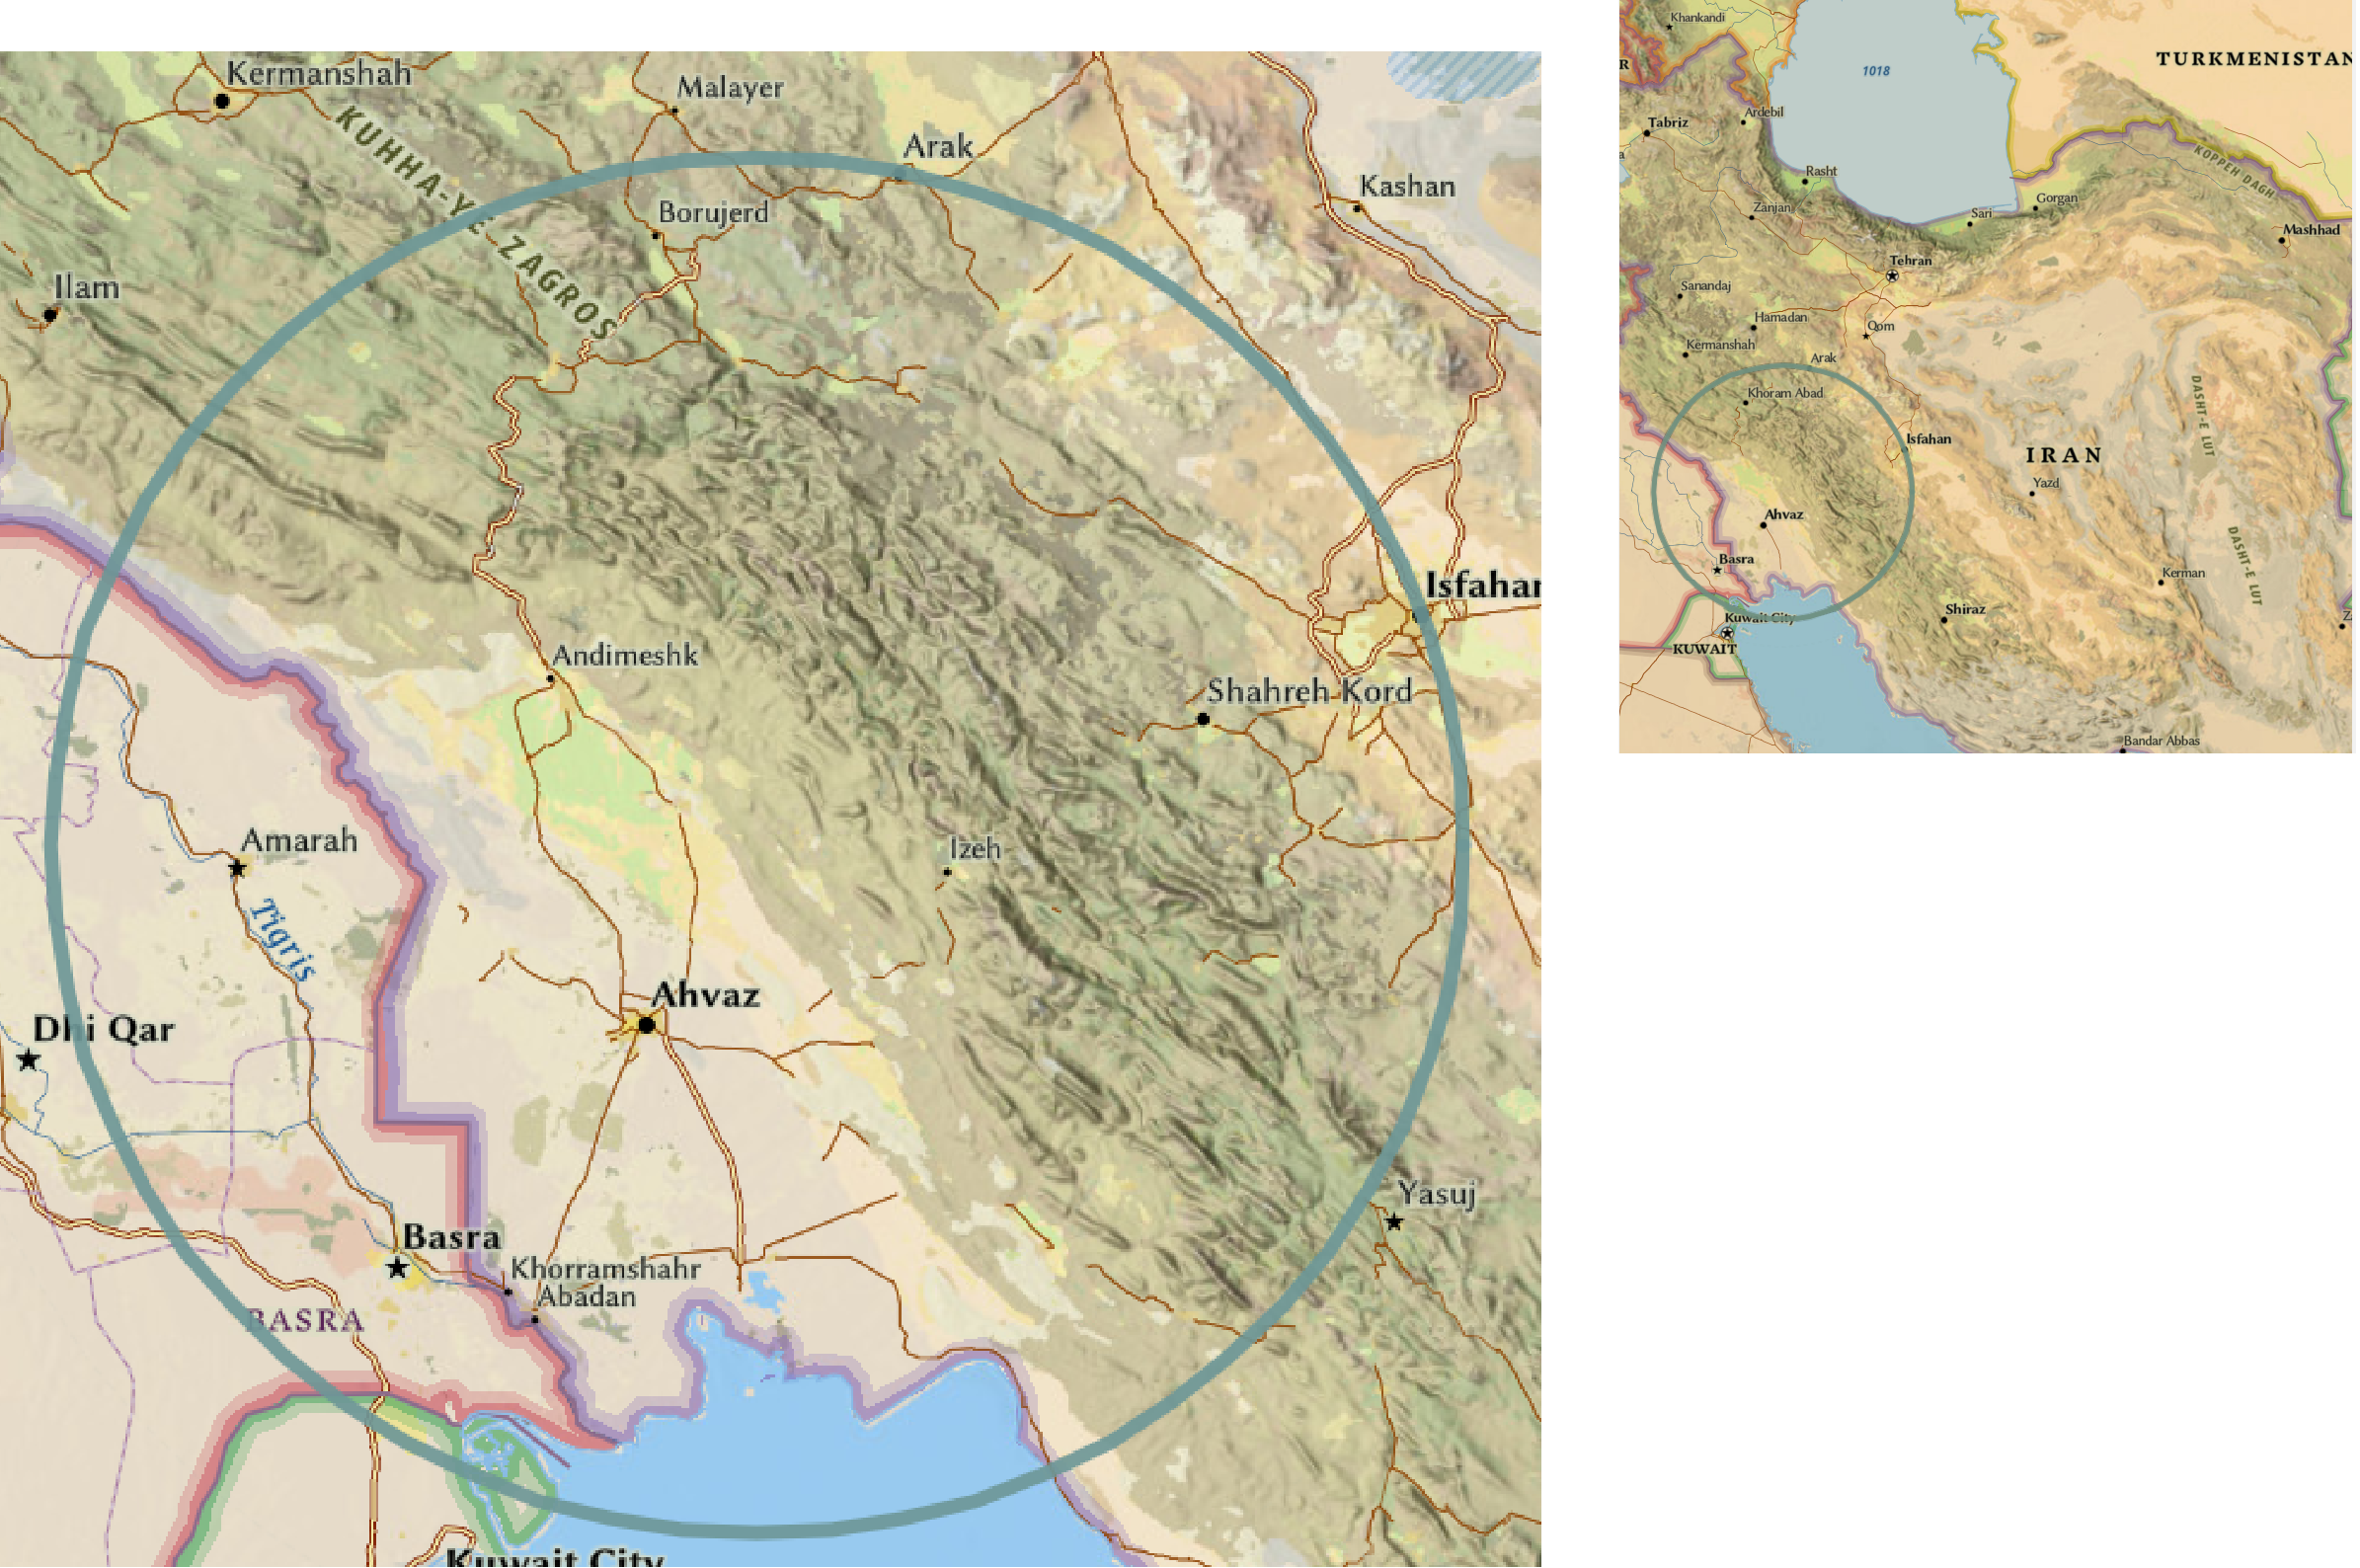
\includegraphics[width=8cm,height=5cm]{Images/reg.png}}\qquad
\subfloat[]
{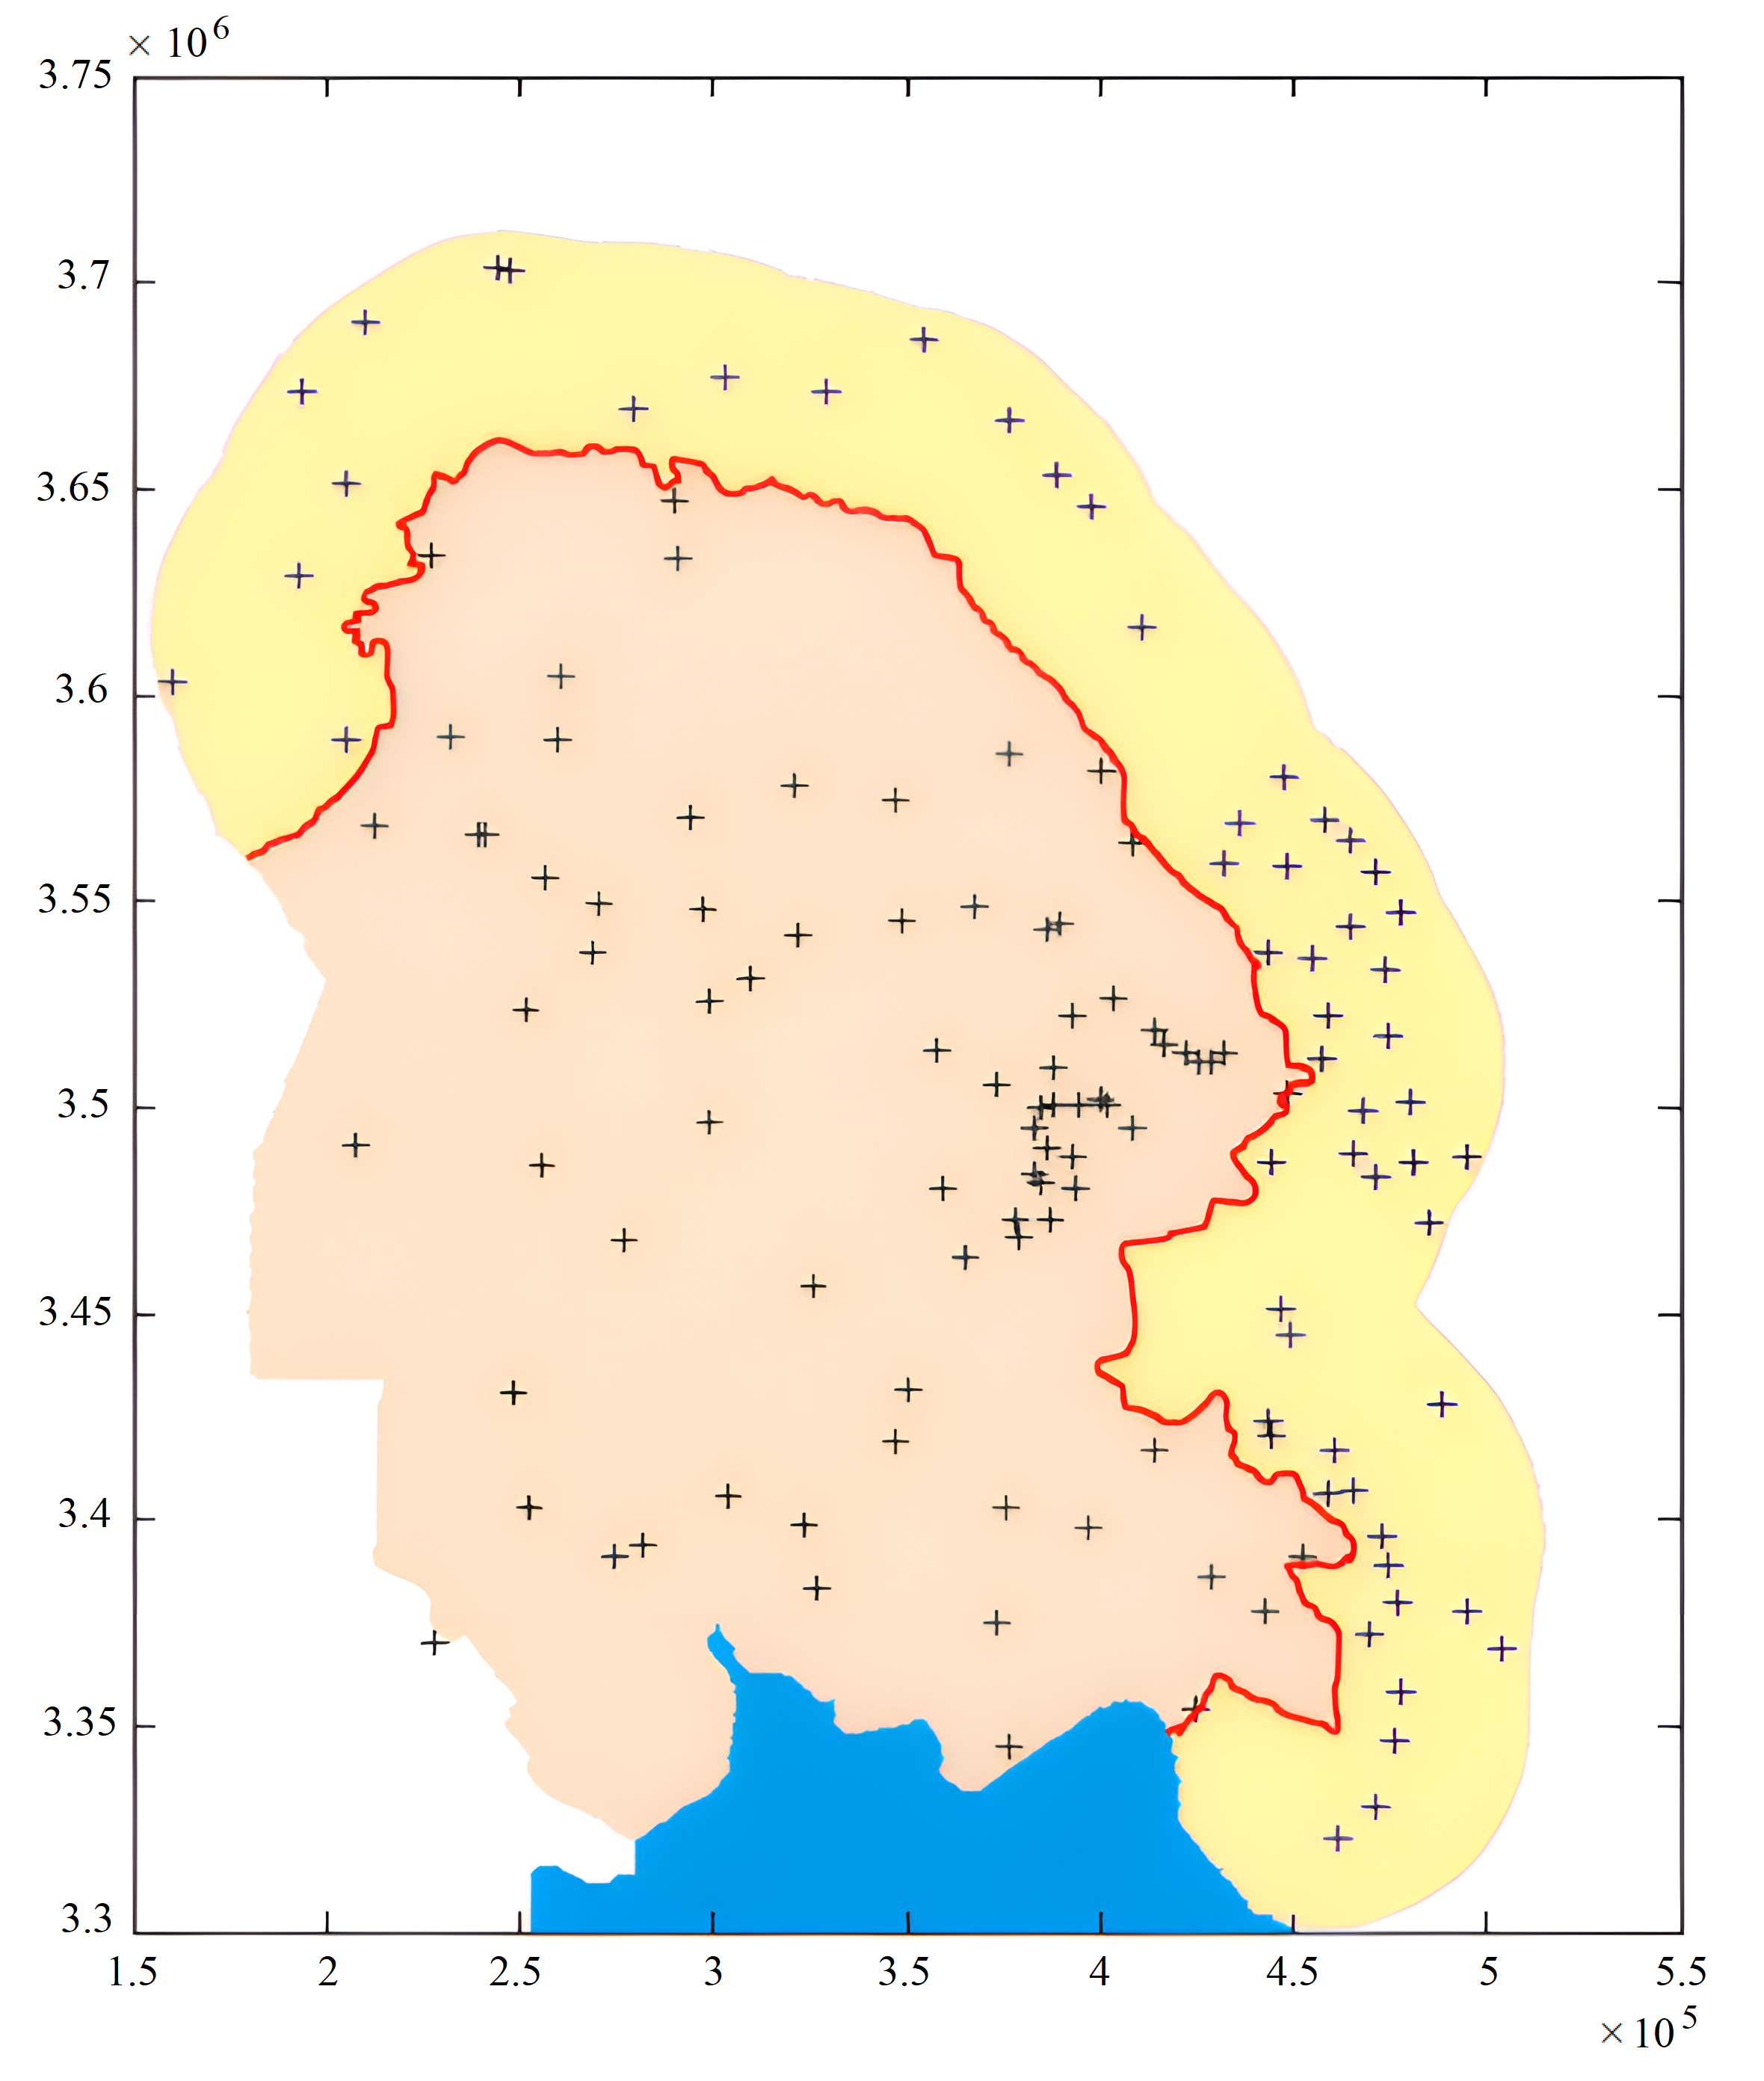
\includegraphics[width=5cm,height=5cm]{Images/studyarea2.png}}
\vspace{-4mm}  
\caption{\footnotesize{(a) Location of Khuzestan Province. (b) Study area including the spatial distribution of rain gauge stations and the 50-kilometer buffer zone.}}\label{fig:location}
\end{center}
\end{figure}
 
The dataset comprises annual mean rainfall measurements collected from 137 stations. A Kolmogorov-Smirnov test yielded a p-value of $0.2896$, confirming that the data approximately follow a normal distribution. As illustrated by the scatter plots in Figure \ref{fig:scatt}, rainfall totals exhibit a positive spatial gradient, increasing gradually from south to north and from west to east. Furthermore, a strong orographic influence is evident, with rainfall intensity increasing in correlation with rising elevation.
\begin{figure}[!ht]
    \begin{center}
        \subfloat[]
            {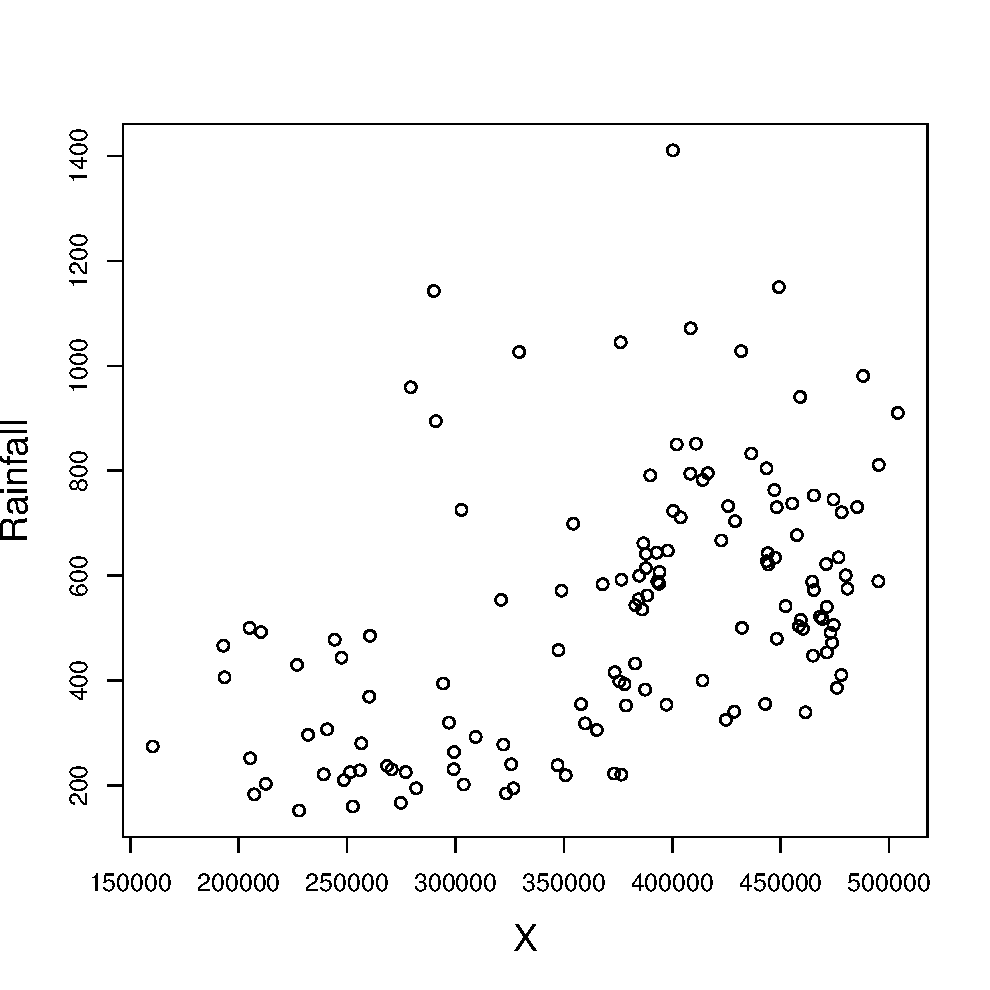
\includegraphics[width=4cm,height=4cm]{Images/plotX-eps-converted-to.pdf}}\quad
            \subfloat[]
             {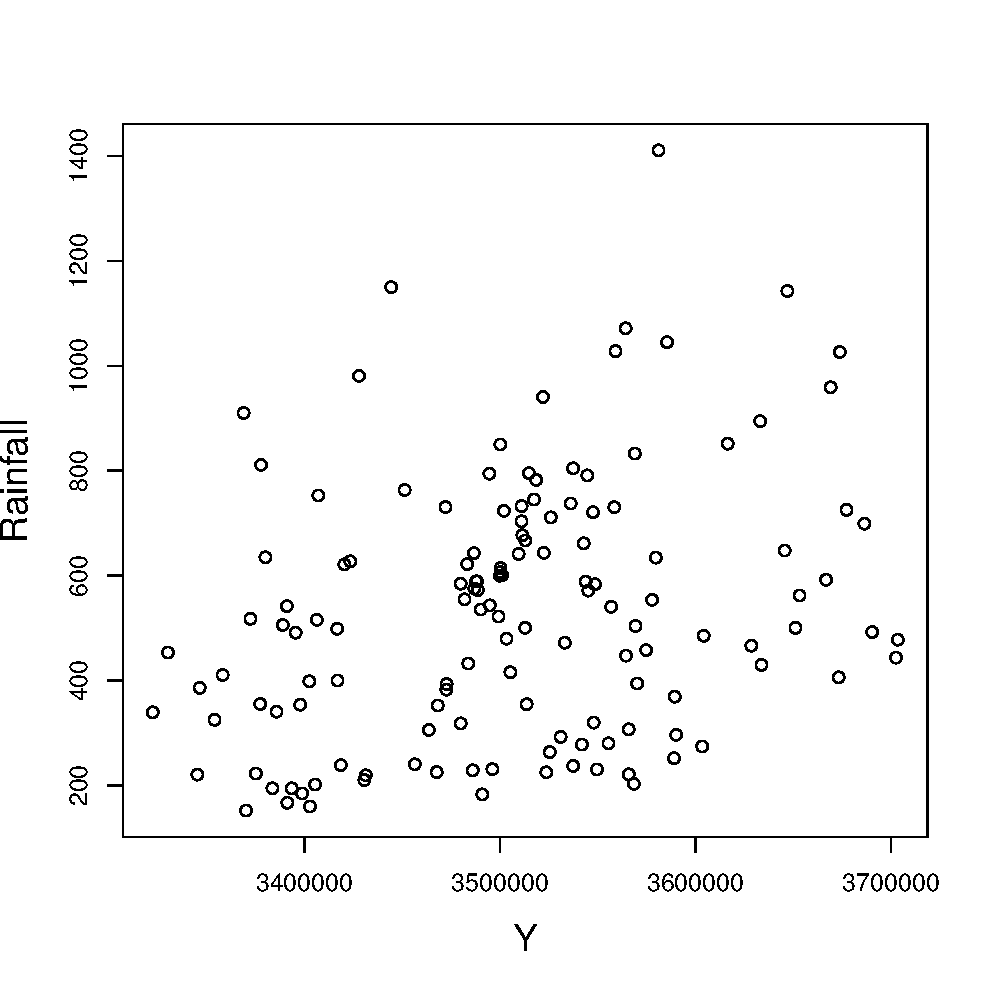
\includegraphics[width=4cm,height=4cm]{Images/plotY-eps-converted-to.pdf}}\quad
             \subfloat[]
            {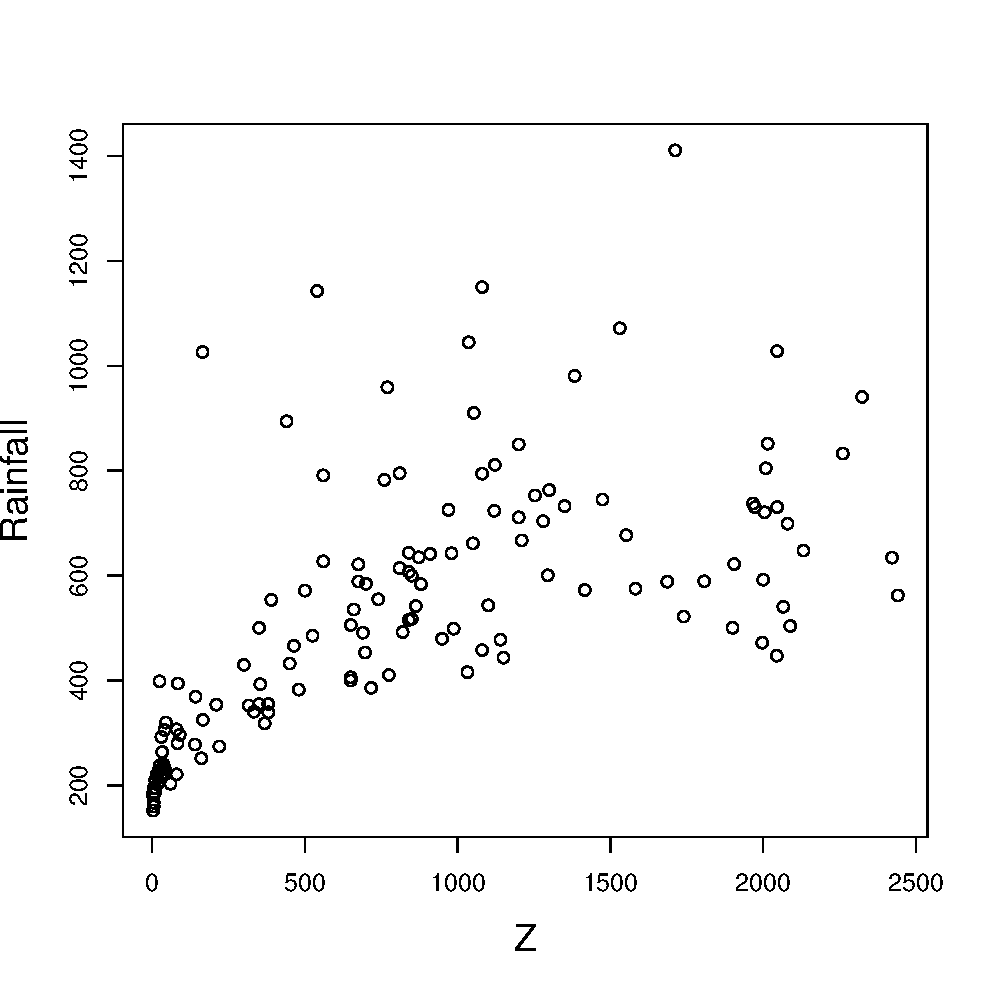
\includegraphics[width=4cm,height=4cm]{Images/plotZ-eps-converted-to.pdf}}
            \vspace{-4mm}        
            \caption{Scatter plot of rainfall data against geographic coordinates (a) Longitude (b) Latitude (c) Elevation.}
             \label{fig:scatt}
    \end{center}    
\end{figure}
A robust regression model (adjusted $R^2 = 0.6047$) was fitted using the MM-type robust regression estimator \citep{Yohai:1991} to remove trends:
\begin{equation}\label{eq:trend}
\hat{\mu}(\mathbf{s}) = -7368.2950 + 0.0048X + 0.0020Y - 0.7042 \times 10^{-9}XY - 2.2519 \times 10^{-5}Z^2.
\end{equation}
After detrending, a spherical isotropic semivariogram is fitted, with approximate similarity across four directions ($0^\circ, 45^\circ, 90^\circ, 135^\circ$) confirming isotropy:
\begin{eqnarray}\label{eq:variogram}
\gamma(h) =\left\{
\begin{tabular}{ll}
0, & $\|h\| = 0$,\\
$c_0 + c_1\!\left(\tfrac{3}{2}\tfrac{\|h\|}{a} - \tfrac{1}{2}\tfrac{\|h\|^3}{a^3}\right)$, & $0 < \|h\| \leq a,\; h \in \mathbb{R}^2$,\\
$c_0 + c_1, $& $\|h\| > a$,
\end{tabular}
\right.
\end{eqnarray}
where $a = 73525.080$, $c_0 = 2434.607$, and $c_1 = 22528.548$.
 
\section{Problem Statement}
 
The optimization is framed as a spatial bi-objective problem designed to resolve the tension between monitoring precision and fiscal constraint. The two competing objectives are: a. Minimizing the Root Mean Total Error (RMTE) to maximize predictive accuracy.  b. Minimizing the total number of stations ($n$) to reduce infrastructure and maintenance costs. Given a finite set of rain gauge locations $\mathbf{s} = \{s_1, \ldots, s_n\}$ within the study domain $\mathcal{B} \subset \mathbb{R}^2$, the Ordinary Kriging prediction at an unobserved location $s_0$ is defined as $\tilde{Z}(s_0|\theta) = \lambda^T z$. Here, the vector of kriging weights, $\lambda$, is obtained by solving the system $\lambda = A^{-1}d$, where
\begin{equation}\label{eq:kriging}
A = \begin{bmatrix} \bigl(C(s_i - s_j|\theta)\bigr)_{i,j=1}^n & \vec{1} \\ \vec{1}^T & 0 \end{bmatrix}, \quad
d = \begin{pmatrix} \bigl(C(s_0 - s_i|\theta)\bigr)_{i=1}^n \\ 1 \end{pmatrix}.
\end{equation}
The ordinary kriging variance at an unobserved location $s_0$ is expressed as: $\sigma^2_{\text{OK}}(s_0) = C(0|\theta) - \lambda^T d$.
To ensure a more robust evaluation, the framework accounts for spatial model parameter uncertainty, acknowledging that the variogram parameters ($\theta$) are typically estimated and not known a priori  %\citep{Marchant:2007, Wadoux:2019}:
\citep{Wadoux:2019}:
\begin{equation}\label{eq:paramunc}
E[\tau^2(s_0)] = \sum_{i=1}^{q}\sum_{j=1}^{q} \text{Cov}(\theta_i,\theta_j) \frac{\partial \lambda^T}{\partial \theta_i} C \frac{\partial \lambda}{\partial \theta_j},
\end{equation}
where $\text{Cov}(\theta_i,\theta_j) \approx F^{-1}(\theta_i,\theta_j)$ via the Fisher information matrix . %\citep{Kitanidis:1987}. Consequently, the total prediction error and its corresponding spatial average across the study domain are defined as:
\begin{equation}\label{eq:totalerror}
\sigma^2_P(s_0, \mathbf{s}) = \sigma^2_{\text{OK}}(s_0, \mathbf{s}) + E[\tau^2(s_0, \mathbf{s})], \qquad
\bar{\sigma}^2_P(\mathbf{s}) = \frac{1}{|\mathcal{B}|} \int_{s_0 \in \mathcal{B}} \sigma^2_P(s_0, \mathbf{s})\, ds_0,
\end{equation}
The Root Mean Total Error (RMTE) is subsequently derived as $\text{RMTE} = \sqrt{\bar{\sigma}^2_P(\mathbf{s})}$, which is computed through numerical integration over the domain. To ensure the optimized network adheres to international benchmarks, the model incorporates World Meteorological Organization (WMO) standards. These standards prescribe a minimum network density of one station per $900\,\text{km}^2$ (minimum spacing $\geq 30\,\text{km}$) for plain areas and one station per $250\,\text{km}^2$ (minimum spacing $\geq 16\,\text{km}$) for mountainous regions. Consequently, the spatial bi-objective optimization problem is formulated as follows:
\begin{equation}\label{eq:problem}
\min_{\mathbf{s} \subset \mathcal{B}}\; f(\mathbf{s}) = (\text{RMTE},\; n), \quad \text{s.t.} \;
\left\{
\begin{tabular}{ll}
$\|s_i - s_j\| \geq 30$, & $s_i, s_j \in P,\; i \neq j$,\\
$\|s_i - s_j\| \geq 16$, & $s_i, s_j \in M,\; i \neq j$,
\end{tabular}
\right.
\end{equation}
where $M$ and $P$ represent the sets of potential station locations in mountainous and plain regions, respectively, and $n$ denotes the total number of stations in the configuration $\mathbf{s}$.
 
\section{HAN Algorithm for Optimal Rain Gauge Network Design}

A Multi-objective Optimization Problem (MOP) is formally defined as $\min f(x) = (f_1(x), \ldots, f_m(x))$ subject to $g_j(x) \leq 0$ for $x \in X \subseteq \mathbb{R}^n$, where $m > 1$. A solution $\hat{x} \in S$ is classified as a Pareto point if there exists no other $x \in S$ such that $f_k(x) \leq f_k(\hat{x})$ for all $k \in \{1, \ldots, m\}$ and $f_i(x) < f_i(\hat{x})$ for at least one objective $i$ \citep{Ehrgott:2005}. The collective set of these non-dominated solutions constitutes the Pareto frontier.

%The HAN Algorithm:
To solve this spatial problem, we employ the HAN algorithm \citep{Lotfian:2023}, which hybridizes the Archived Multi-Objective Simulated Annealing (AMOSA) \citep{Bandyopadhyay:2008} and the Non-dominated Sorting Genetic Algorithm II (NSGA-II) \citep{Deb:2002}. The algorithm maintains two distinct memory structures: the Archive (storing solutions generated via AMOSA) and the Pop (storing elite Pareto solutions produced through genetic operators). By applying NSGA-II’s crossover and mutation to the Archive members, the algorithm effectively integrates the rigorous local search of simulated annealing with the robust global exploration of evolutionary strategies. The domination intensity between two solutions $a$ and $b$ is quantified as:
\begin{equation*}
	\Delta\text{dom}\{a,b\} = \prod{\substack{i=1 \ f_i(a) \neq f_i(b)}}^{m} \frac{|f_i(a) - f_i(b)|}{R_i},
\end{equation*}
where $R_i$ represents the range of the $i$-th objective. The algorithm's performance is governed by several hyper-parameters: initial and final temperatures ($T_{\max}, T_{\min}$), inner iterations per temperature step ($InIter$), initial archive size ($CL$), soft and hard limits ($SL, HL$), the cooling rate ($\alpha \in [0.5, 0.99]$), and genetic probabilities ($P_c, P_m$). These parameters are optimized using the Taguchi method to ensure robust convergence \citep{Taguchi:1986}.

%Discretization and Initialization:
The study area is discretized into $10{,}000$ potential station locations. To approximate the spatial average error, the integral in \eqref{eq:totalerror} is evaluated numerically across a $14 \times 12$ regular grid (168 prediction points). The initial population comprises randomly generated networks containing between 100 and 137 stations, each represented as a coordinate matrix adhering to the distance constraints defined in \eqref{eq:problem}. During each iteration, candidate networks are generated by perturbing existing station locations. To ensure exhaustive local exploration, $InIter$ is set equal to the total number of stations, allowing each station to be perturbed exactly once per inner loop. When the Archive size exceeds the hard limit ($HL$), it is thinned using single-linkage clustering to maintain diversity. Upon termination, the Archive and Pop are merged, re-sorted based on non-dominance and crowding distance, and the final Pareto frontier is extracted.
 
\section{Experimental Results}
 The HAN algorithm parameters were calibrated using the Taguchi method to ensure optimal performance, resulting in the following configuration: $\text{SL} = 50$, $\text{HL} = 40$, $\alpha = 0.99$, $P_c = 0.90$, $P_m = 0.20$, and $\text{MaxIt} = 800$.  
\begin{figure}[!ht]
\begin{center}
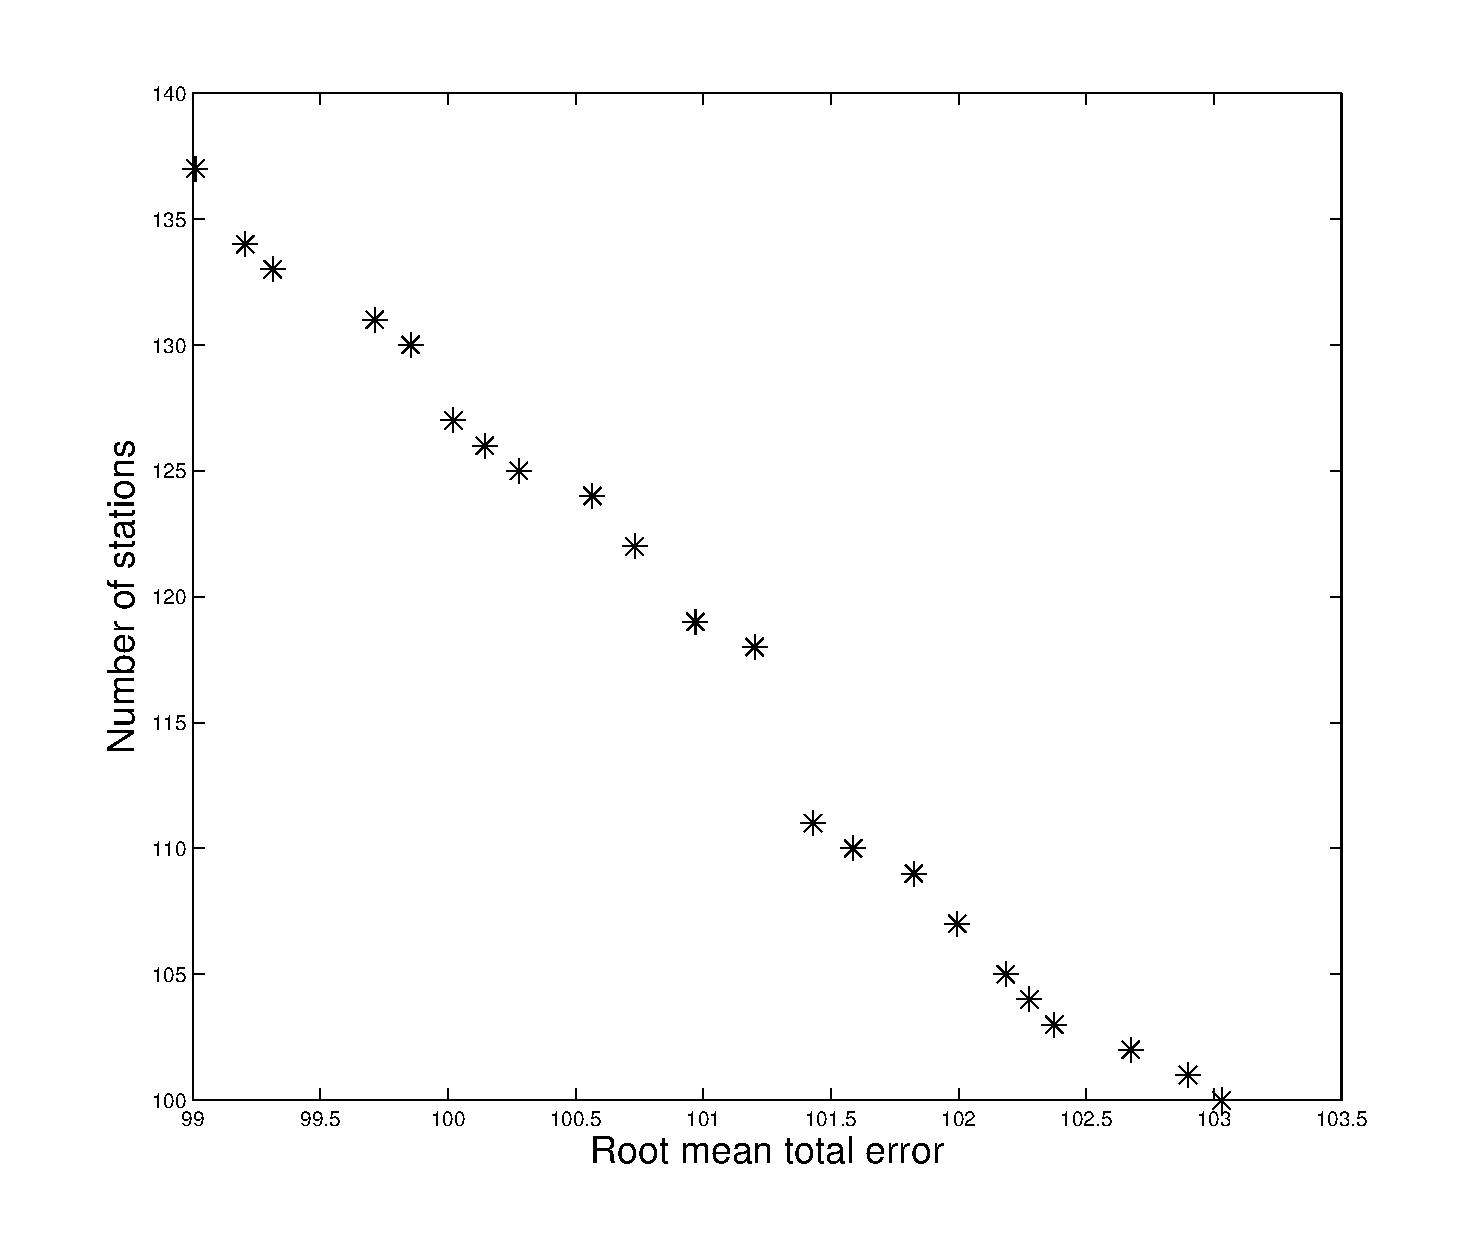
\includegraphics[width=6cm]{Images/khfront-eps-converted-to.pdf}
\vspace{-6mm}  
\caption{\footnotesize{The Pareto frontier estimated by the HAN algorithm.}}\label{fig:pareto}
\end{center}
\end{figure}
Figure \ref{fig:pareto} illustrates the estimated Pareto frontier, which clearly depicts the competitive trade-off between the Root Mean Total Error (RMTE) and the total number of stations ($n$). To further analyze the results, Figure \ref{fig:networks} displays four selected optimal network configurations. In these visualizations, brown and green regions differentiate the mountainous and plain topographies, respectively, illustrating how the algorithm adapts station density according to regional constraints and spatial variance.
\begin{figure}[!ht]
	\begin{center}
		\subfloat[]
		{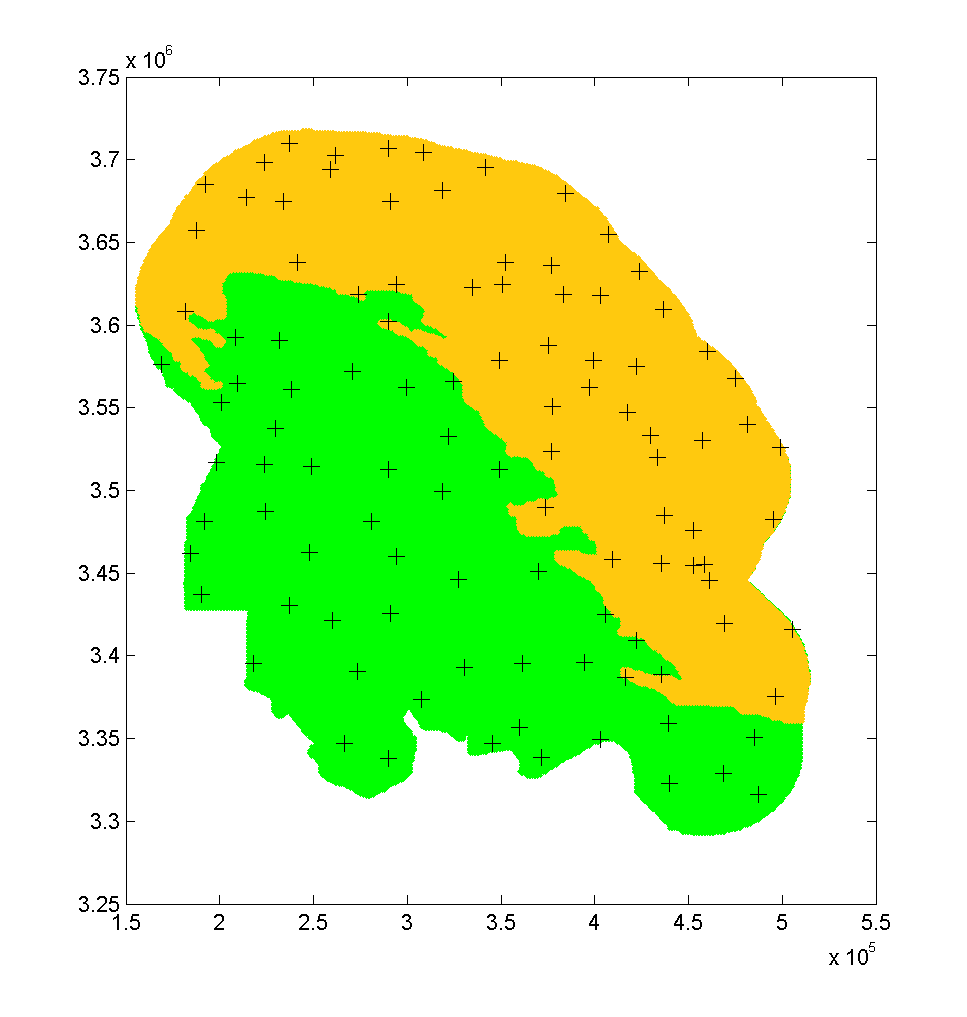
\includegraphics[width=3.8cm,height=4cm]{Images/105-eps-converted-to.pdf}}
		\subfloat[]
		{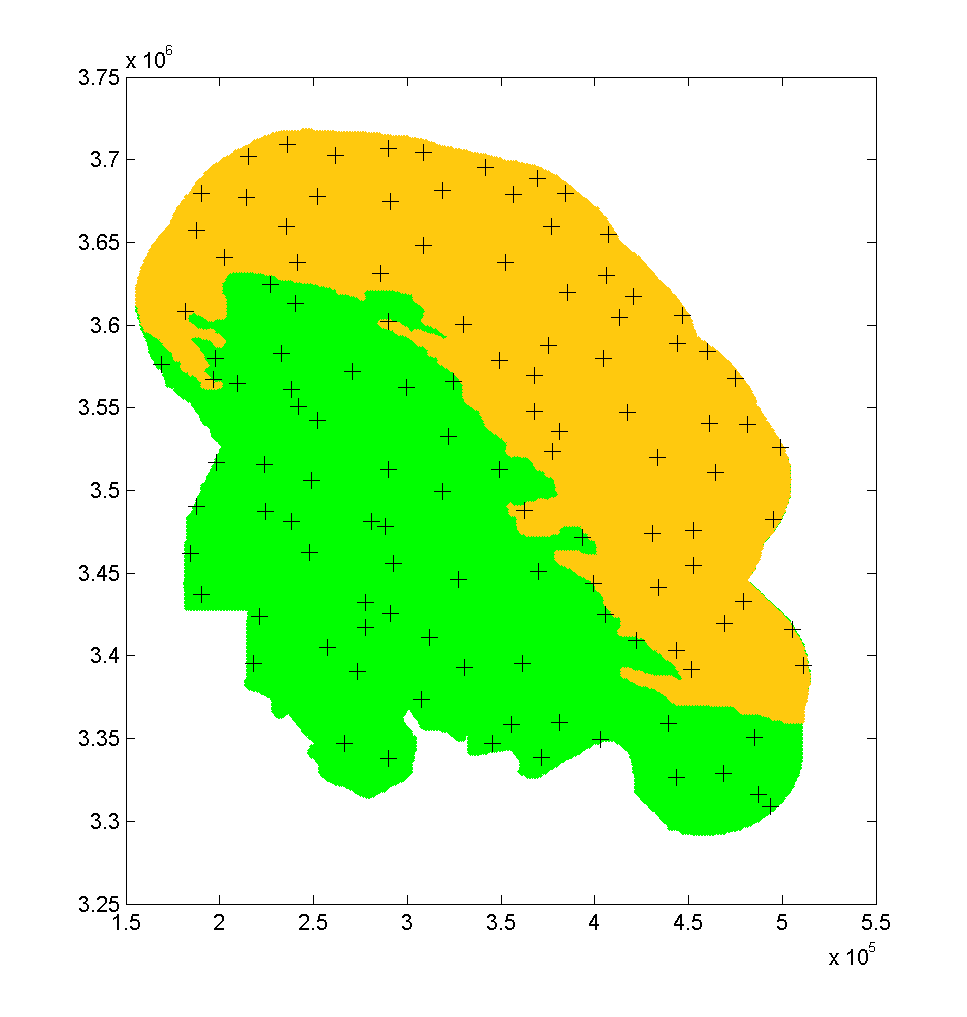
\includegraphics[width=3.8cm,height=4cm]{Images/118-eps-converted-to.pdf}}
		\subfloat[]
		{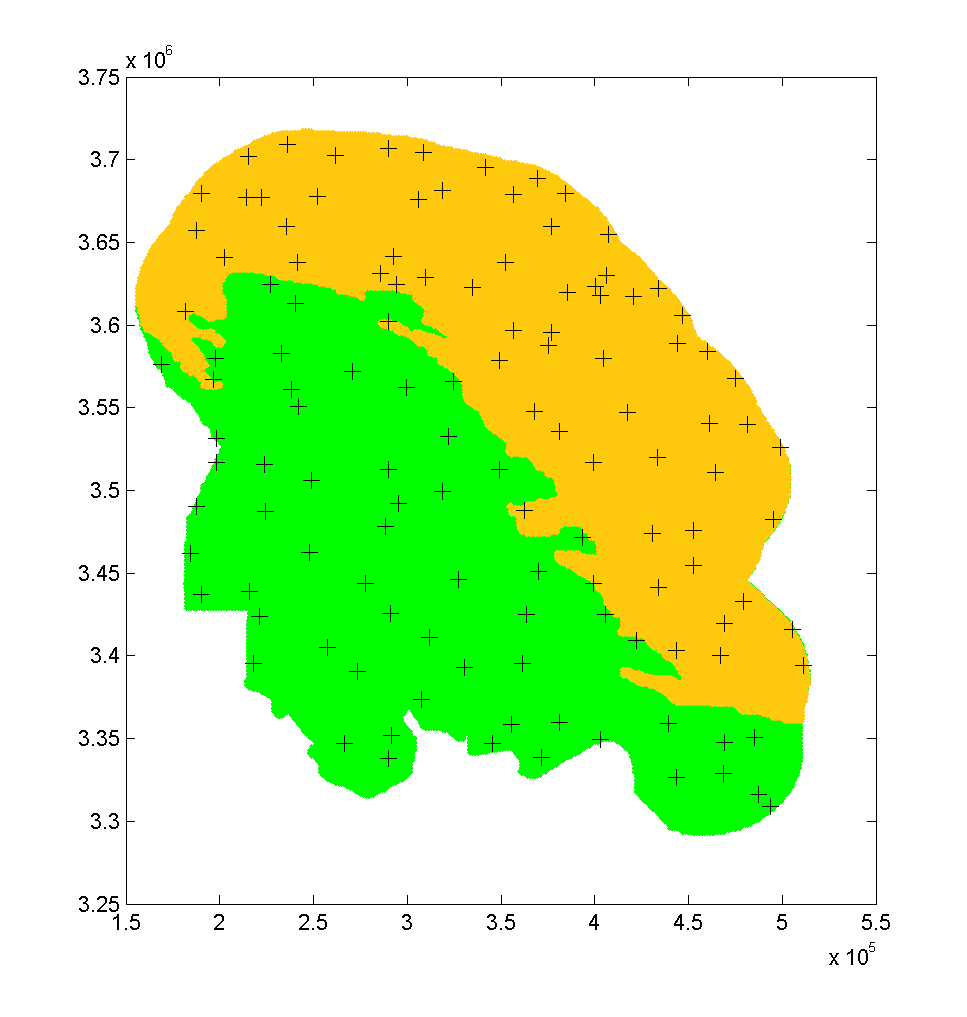
\includegraphics[width=3.8cm,height=4cm]{Images/124-eps-converted-to.pdf}}
		\subfloat[]
		{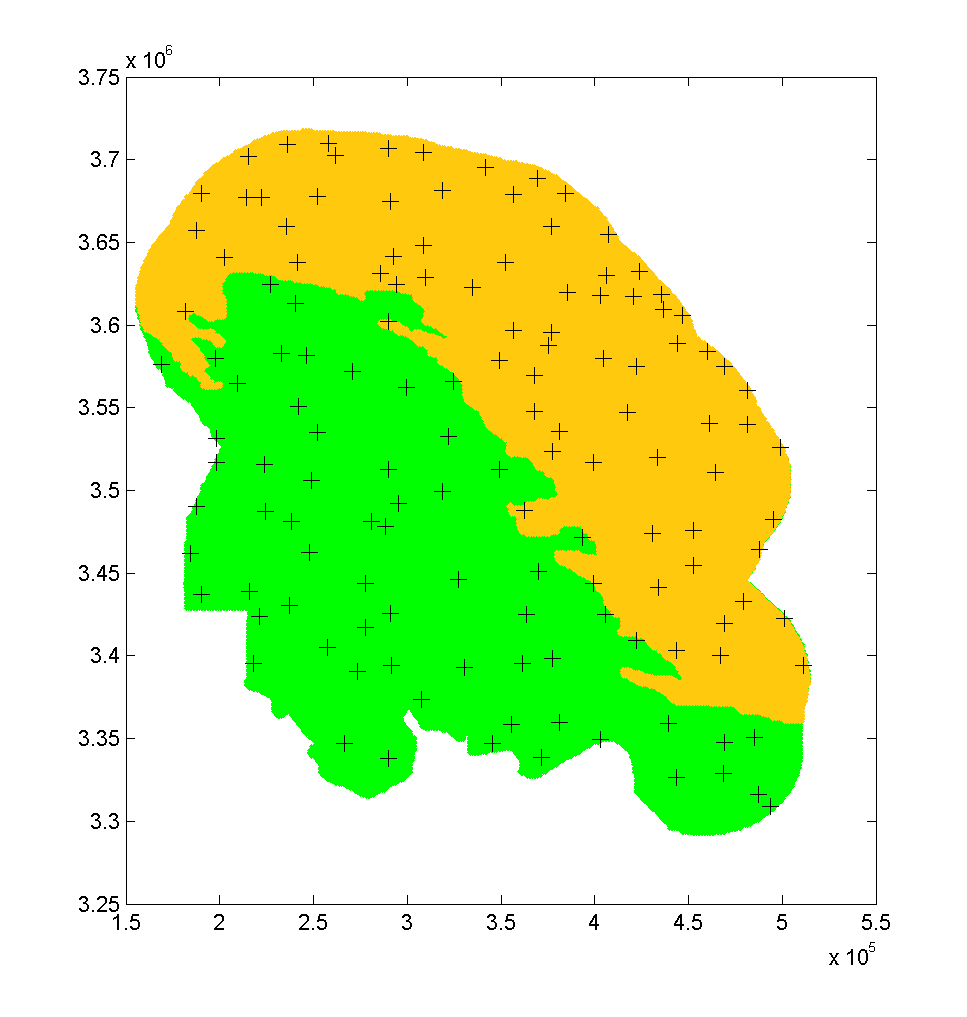
\includegraphics[width=3.8cm,height=4cm]{Images/137-eps-converted-to.pdf}}\vspace{-4mm}        
		\caption{\footnotesize{Optimal rain gauge station networks obtained by the HAN algorithm: (a) 105 stations, (b) 118 stations, (c) 124 stations, (d) 137 stations.}}
		\label{fig:networks}
	\end{center}    
\end{figure}
 
Table \ref{tab:results} presents a comparative analysis between the existing Ministry of Energy network and the optimal configurations generated by the HAN algorithm. The results demonstrate that all optimized networks achieve a lower RMTE than the current monitoring system, even with a significantly reduced number of stations. Notably, the 105-station optimal configuration reduces the RMTE from $110.27$ to $102.18$ while eliminating 32 redundant stations. Furthermore, the 137-station optimal network—representing the current total capacity—achieves an improvement in predictive accuracy of over $10\%$ relative to the existing network. These findings underscore the substantial efficiency gains achievable through systematic spatial optimization.
\begin{table}[!ht]
\begin{center}
	\caption{Objective function values for the current and optimal networks.}\label{tab:results}
\scriptsize
\begin{tabular}{lcc}
  \hline
  Network & Number of Stations ($n$) & RMTE \\ \hline
  Current network & 137 & 110.2694 \\ [3mm]
   & 105 & 102.1847 \\
  Optimal networks & 118 & 101.2015 \\
   & 124 & 100.5659 \\
   & 137 & 99.0113 \\ \hline
\end{tabular}
\end{center}
\end{table}

 \vspace*{-20mm}
\section*{Conclusion}
This study demonstrates the efficacy of the HAN algorithm within a bi-objective optimization framework for restructuring the rain gauge network in Khuzestan Province, Iran. The comparative analysis reveals that the current network, which evolved incrementally, can be significantly improved in terms of both predictive accuracy and cost efficiency. By strategically reconfiguring station locations, the HAN algorithm identifies designs that utilize fewer stations yet consistently outperform the existing network—effectively reducing operational costs without compromising data reliability. These results provide a robust methodological benchmark for hydrometeorological network planning, particularly in regions facing similar climatic variability and geographical complexities.

\begin{thebibliography}{99}
 
\bibitem[Ali and Othman(2018)]{Ali:2018}
Ali, M.Z.M. and Othman, F., (2018), Raingauge Network Optimization in a Tropical Urban Area by Coupling Cross-Validation with the Geostatistical Technique, {\it Hydrological Sciences Journal}, \textbf{63}(3), 474-491.
 
\bibitem[Bandyopadhyay et al.(2008)]{Bandyopadhyay:2008}
Bandyopadhyay S., Saha S., Maulik U. and Deb K., (2008), A Simulated Annealing-Based Multiobjective Optimization Algorithm: AMOSA, {\it IEEE Transactions on Evolutionary Computation}, \textbf{12}(3), 269-283.
 
\bibitem[Deb et al.(2002)]{Deb:2002}
Deb K., Pratap A., Agarwal S. and Meyarivan T., (2002), A Fast and Elitist Multiobjective Genetic Algorithm: NSGA-II, {\it IEEE Transactions on Evolutionary Computation}, \textbf{6}(2), 182-197.
 
\bibitem[Ehrgott(2005)]{Ehrgott:2005}
Ehrgott M., (2005), {\it Multicriteria Optimization}, Springer, Berlin.
 
\bibitem[Fei et al.(2017)]{Fei:2017}
Fei Z., Li B., Yang S., Xing C., Chen H. and Hanzo L., (2017), A Survey of Multi-Objective Optimization in Wireless Sensor Networks: Metrics, Algorithms, and Open Problems, {\it IEEE Communications Surveys Tutorials}, \textbf{19}(1), 550-586.
 
\bibitem[Kar et al.(2015)]{Kar:2015}
Kar A.K., Lohani A.K., Goel N.K. and Roy G.P., (2015), Rain Gauge Network Design for Flood Forecasting Using Multi-Criteria Decision Analysis and Clustering Techniques in Lower Mahanadi River Basin, India, {\it Journal of Hydrology: Regional Studies}, \textbf{4}, 313-332.
 
\bibitem[Lotfian and Mohammadzadeh(2023)]{Lotfian:2023}
Lotfian E. and Mohammadzadeh M., (2023), Multi-Objective Optimization of Spatial Sampling Using a New Hybrid AMOSA NSGA-II Algorithm, {\it Computational and Applied Mathematics}, \textbf{42}, 24.
 
\bibitem[de Oliveira Simoyama et al.(2022)]{Simoyama:2022}
de Oliveira Simoyama F., Tom\'{a}s L.R., Pinto F.M., Salles-Neto L.L. and Santos L.B.L., (2022), Optimal Rain Gauge Network to Reduce Rainfall Impacts on Urban Mobility, {\it Industrial Management \& Data Systems}, \textbf{122}(10), 2261-2280.
 
\bibitem[de Oliveira Simoyama et al.(2023)]{Simoyama:2023}
de Oliveira Simoyama F., Croope S., de Salles Neto L.L. and Santos L.B.L., (2023), Optimization of Rain Gauge Networks--A Systematic Literature Review, {\it Socio-Economic Planning Sciences}, \textbf{86}, 101469.
 
\bibitem[Taguchi(1986)]{Taguchi:1986}
Taguchi G., (1986), {\it Introduction to Quality Engineering: Designing Quality into Products and Processes}, Asian Productivity Organization, Tokyo.
 
\bibitem[Wadoux et al.(2019)]{Wadoux:2019}
Wadoux A.M.C., Marchant B.P. and Lark R.M., (2019), Efficient Sampling for Geostatistical Surveys, {\it European Journal of Soil Science}, \textbf{70}(5), 975-989.
 
\bibitem[Yohai et al.(1991)]{Yohai:1991}
Yohai V.J., Stahel W.A. and Zamar R.H., (1991), A Procedure for Robust Estimation and Inference in Linear Regression, {\it Directions in Robust Statistics and Diagnostics}, 365-374.
 
\bibitem[Zarei et al. (2025)]{Zarei:2025}
Zarei, M., Sarvestan, R. and Alavinia, S. H., (2025), Optimizing Rain-Gauge Network Design for Enhanced Estimate Rainfall in Ungauged Plain and Mountainous Regions, {\it Earth Science Informatics}, \textbf{18}(2), 219.
 
\bibitem[Zhu and Stein (2006)]{Zhu:2006}
Zhu Z. and Stein M.L., (2006), Spatial Sampling Design for Prediction with Estimated Parameters, {\it Journal of Agricultural, Biological, and Environmental Statistics}, \textbf{11}(1), 24-44.
 
\end{thebibliography}
\end{document} 